
%% bare_conf.tex
%% V1.4b
%% 2015/08/26
%% by Michael Shell
%% See:
%% http://www.michaelshell.org/
%% for current contact information.
%%
%% This is a skeleton file demonstrating the use of IEEEtran.cls
%% (requires IEEEtran.cls version 1.8b or later) with an IEEE
%% conference paper.
%%
%% Support sites:
%% http://www.michaelshell.org/tex/ieeetran/
%% http://www.ctan.org/pkg/ieeetran
%% and
%% http://www.ieee.org/

%%*************************************************************************
%% Legal Notice:
%% This code is offered as-is without any warranty either expressed or
%% implied; without even the implied warranty of MERCHANTABILITY or
%% FITNESS FOR A PARTICULAR PURPOSE! 
%% User assumes all risk.
%% In no event shall the IEEE or any contributor to this code be liable for
%% any damages or losses, including, but not limited to, incidental,
%% consequential, or any other damages, resulting from the use or misuse
%% of any information contained here.
%%
%% All comments are the opinions of their respective authors and are not
%% necessarily endorsed by the IEEE.
%%
%% This work is distributed under the LaTeX Project Public License (LPPL)
%% ( http://www.latex-project.org/ ) version 1.3, and may be freely used,
%% distributed and modified. A copy of the LPPL, version 1.3, is included
%% in the base LaTeX documentation of all distributions of LaTeX released
%% 2003/12/01 or later.
%% Retain all contribution notices and credits.
%% ** Modified files should be clearly indicated as such, including  **
%% ** renaming them and changing author support contact information. **
%%*************************************************************************


% *** Authors should verify (and, if needed, correct) their LaTeX system  ***
% *** with the testflow diagnostic prior to trusting their LaTeX platform ***
% *** with production work. The IEEE's font choices and paper sizes can   ***
% *** trigger bugs that do not appear when using other class files.       ***                          ***
% The testflow support page is at:
% http://www.michaelshell.org/tex/testflow/



\documentclass[conference]{IEEEtran}
% Some Computer Society conferences also require the compsoc mode option,
% but others use the standard conference format.
%
% If IEEEtran.cls has not been installed into the LaTeX system files,
% manually specify the path to it like:
% \documentclass[conference]{../sty/IEEEtran}





% Some very useful LaTeX packages include:
% (uncomment the ones you want to load)


% *** MISC UTILITY PACKAGES ***
%
%\usepackage{ifpdf}
% Heiko Oberdiek's ifpdf.sty is very useful if you need conditional
% compilation based on whether the output is pdf or dvi.
% usage:
% \ifpdf
%   % pdf code
% \else
%   % dvi code
% \fi
% The latest version of ifpdf.sty can be obtained from:
% http://www.ctan.org/pkg/ifpdf
% Also, note that IEEEtran.cls V1.7 and later provides a builtin
% \ifCLASSINFOpdf conditional that works the same way.
% When switching from latex to pdflatex and vice-versa, the compiler may
% have to be run twice to clear warning/error messages.






% *** CITATION PACKAGES ***
%
\usepackage{cite}
% cite.sty was written by Donald Arseneau
% V1.6 and later of IEEEtran pre-defines the format of the cite.sty package
% \cite{} output to follow that of the IEEE. Loading the cite package will
% result in citation numbers being automatically sorted and properly
% "compressed/ranged". e.g., [1], \cite{rubinsztejn_framework_2005}, \cite{gamma_design_1995}, \cite{holder_system_1999}, \cite{pratikakis_transparent_2004}, \cite{_fusion_????} without using
% cite.sty will become [1], \cite{gamma_design_1995}, \cite{pratikakis_transparent_2004}--\cite{holder_system_1999}, \cite{rubinsztejn_framework_2005} using cite.sty. cite.sty's
% \cite will automatically add leading space, if needed. Use cite.sty's
% noadjust option (cite.sty V3.8 and later) if you want to turn this off
% such as if a citation ever needs to be enclosed in parenthesis.
% cite.sty is already installed on most LaTeX systems. Be sure and use
% version 5.0 (2009-03-20) and later if using hyperref.sty.
% The latest version can be obtained at:
% http://www.ctan.org/pkg/cite
% The documentation is contained in the cite.sty file itself.






% *** GRAPHICS RELATED PACKAGES ***
%
\ifCLASSINFOpdf
  \usepackage[pdftex]{graphicx}
  % declare the path(s) where your graphic files are
  % \graphicspath{{../pdf/}{../jpeg/}}
  % and their extensions so you won't have to specify these with
  % every instance of \includegraphics
  \DeclareGraphicsExtensions{.pdf,.jpeg,.png}
\else
  % or other class option (dvipsone, dvipdf, if not using dvips). graphicx
  % will default to the driver specified in the system graphics.cfg if no
  % driver is specified.
  \usepackage[dvips]{graphicx}
  % declare the path(s) where your graphic files are
  % \graphicspath{{../eps/}}
  % and their extensions so you won't have to specify these with
  % every instance of \includegraphics
  \DeclareGraphicsExtensions{.eps}
\fi
% graphicx was written by David Carlisle and Sebastian Rahtz. It is
% required if you want graphics, photos, etc. graphicx.sty is already
% installed on most LaTeX systems. The latest version and documentation
% can be obtained at: 
% http://www.ctan.org/pkg/graphicx
% Another good source of documentation is "Using Imported Graphics in
% LaTeX2e" by Keith Reckdahl which can be found at:
% http://www.ctan.org/pkg/epslatex
%
% latex, and pdflatex in dvi mode, support graphics in encapsulated
% postscript (.eps) format. pdflatex in pdf mode supports graphics
% in .pdf, .jpeg, .png and .mps (metapost) formats. Users should ensure
% that all non-photo figures use a vector format (.eps, .pdf, .mps) and
% not a bitmapped formats (.jpeg, .png). The IEEE frowns on bitmapped formats
% which can result in "jaggedy"/blurry rendering of lines and letters as
% well as large increases in file sizes.
%
% You can find documentation about the pdfTeX application at:
% http://www.tug.org/applications/pdftex





% *** MATH PACKAGES ***
%
\usepackage[fleqn]{amsmath}
% A popular package from the American Mathematical Society that provides
% many useful and powerful commands for dealing with mathematics.
%
% Note that the amsmath package sets \interdisplaylinepenalty to 10000
% thus preventing page breaks from occurring within multiline equations. Use:
%\interdisplaylinepenalty=2500
% after loading amsmath to restore such page breaks as IEEEtran.cls normally
% does. amsmath.sty is already installed on most LaTeX systems. The latest
% version and documentation can be obtained at:
% http://www.ctan.org/pkg/amsmath




% *** MATH PACKAGES ***
%
\usepackage{amssymb}





% *** SPECIALIZED LIST PACKAGES ***
%
\usepackage{algorithmic}
% algorithmic.sty was written by Peter Williams and Rogerio Brito.
% This package provides an algorithmic environment fo describing algorithms.
% You can use the algorithmic environment in-text or within a figure
% environment to provide for a floating algorithm. Do NOT use the algorithm
% floating environment provided by algorithm.sty (by the same authors) or
% algorithm2e.sty (by Christophe Fiorio) as the IEEE does not use dedicated
% algorithm float types and packages that provide these will not provide
% correct IEEE style captions. The latest version and documentation of
% algorithmic.sty can be obtained at:
% http://www.ctan.org/pkg/algorithms
% Also of interest may be the (relatively newer and more customizable)
% algorithmicx.sty package by Szasz Janos:
% http://www.ctan.org/pkg/algorithmicx




% *** ALIGNMENT PACKAGES ***
%
\usepackage{array}
% Frank Mittelbach's and David Carlisle's array.sty patches and improves
% the standard LaTeX2e array and tabular environments to provide better
% appearance and additional user controls. As the default LaTeX2e table
% generation code is lacking to the point of almost being broken with
% respect to the quality of the end results, all users are strongly
% advised to use an enhanced (at the very least that provided by array.sty)
% set of table tools. array.sty is already installed on most systems. The
% latest version and documentation can be obtained at:
% http://www.ctan.org/pkg/array


% IEEEtran contains the IEEEeqnarray family of commands that can be used to
% generate multiline equations as well as matrices, tables, etc., of high
% quality.




% *** SUBFIGURE PACKAGES ***
\ifCLASSOPTIONcompsoc
  \usepackage[caption=false,font=normalsize,labelfont=sf,textfont=sf]{subfig}
\else
  \usepackage[caption=false,font=footnotesize]{subfig}
\fi
% subfig.sty, written by Steven Douglas Cochran, is the modern replacement
% for subfigure.sty, the latter of which is no longer maintained and is
% incompatible with some LaTeX packages including fixltx2e. However,
% subfig.sty requires and automatically loads Axel Sommerfeldt's caption.sty
% which will override IEEEtran.cls' handling of captions and this will result
% in non-IEEE style figure/table captions. To prevent this problem, be sure
% and invoke subfig.sty's "caption=false" package option (available since
% subfig.sty version 1.3, 2005/06/28) as this is will preserve IEEEtran.cls
% handling of captions.
% Note that the Computer Society format requires a larger sans serif font
% than the serif footnote size font used in traditional IEEE formatting
% and thus the need to invoke different subfig.sty package options depending
% on whether compsoc mode has been enabled.
%
% The latest version and documentation of subfig.sty can be obtained at:
% http://www.ctan.org/pkg/subfig




% *** FLOAT PACKAGES ***
%
\usepackage{fixltx2e}
% fixltx2e, the successor to the earlier fix2col.sty, was written by
% Frank Mittelbach and David Carlisle. This package corrects a few problems
% in the LaTeX2e kernel, the most notable of which is that in current
% LaTeX2e releases, the ordering of single and double column floats is not
% guaranteed to be preserved. Thus, an unpatched LaTeX2e can allow a
% single column figure to be placed prior to an earlier double column
% figure.
% Be aware that LaTeX2e kernels dated 2015 and later have fixltx2e.sty's
% corrections already built into the system in which case a warning will
% be issued if an attempt is made to load fixltx2e.sty as it is no longer
% needed.
% The latest version and documentation can be found at:
% http://www.ctan.org/pkg/fixltx2e


\usepackage{stfloats}
% stfloats.sty was written by Sigitas Tolusis. This package gives LaTeX2e
% the ability to do double column floats at the bottom of the page as well
% as the top. (e.g., "\begin{figure*}[!b]" is not normally possible in
% LaTeX2e). It also provides a command:
%\fnbelowfloat
% to enable the placement of footnotes below bottom floats (the standard
% LaTeX2e kernel puts them above bottom floats). This is an invasive package
% which rewrites many portions of the LaTeX2e float routines. It may not work
% with other packages that modify the LaTeX2e float routines. The latest
% version and documentation can be obtained at:
% http://www.ctan.org/pkg/stfloats
% Do not use the stfloats baselinefloat ability as the IEEE does not allow
% \baselineskip to stretch. Authors submitting work to the IEEE should note
% that the IEEE rarely uses double column equations and that authors should try
% to avoid such use. Do not be tempted to use the cuted.sty or midfloat.sty
% packages (also by Sigitas Tolusis) as the IEEE does not format its papers in
% such ways.
% Do not attempt to use stfloats with fixltx2e as they are incompatible.
% Instead, use Morten Hogholm'a dblfloatfix which combines the features
% of both fixltx2e and stfloats:
%
% \usepackage{dblfloatfix}
% The latest version can be found at:
% http://www.ctan.org/pkg/dblfloatfix




% *** PDF, URL AND HYPERLINK PACKAGES ***
%
\usepackage{url}
% url.sty was written by Donald Arseneau. It provides better support for
% handling and breaking URLs. url.sty is already installed on most LaTeX
% systems. The latest version and documentation can be obtained at:
% http://www.ctan.org/pkg/url
% Basically, \url{my_url_here}.



\usepackage{hyperref}

\usepackage{minted}
\usepackage{tcolorbox}
\usepackage{etoolbox}
\BeforeBeginEnvironment{minted}{\begin{tcolorbox}}%
\AfterEndEnvironment{minted}{\end{tcolorbox}}%
\AtBeginEnvironment{minted}{\fontsize{8}{8}}




%
% Digunakan untuk membuat inline list dan numbering
\usepackage{paralist}




%
% 
\usepackage{algorithm}
\usepackage{algorithmic}




%
% Digunakan untuk membuat tabel yang panjang, lebih dari 1 halaman
%
\usepackage{longtable, supertabular, booktabs}
  \newcommand{\ra}[1]{\renewcommand{\arraystretch}{#1}}




% *** Do not adjust lengths that control margins, column widths, etc. ***
% *** Do not use packages that alter fonts (such as pslatex).         ***
% There should be no need to do such things with IEEEtran.cls V1.6 and later.
% (Unless specifically asked to do so by the journal or conference you plan
% to submit to, of course. )


% correct bad hyphenation here
\hyphenation{op-tical net-works semi-conduc-tor}


\begin{document}
%
% paper title
% Titles are generally capitalized except for words such as a, an, and, as,
% at, but, by, for, in, nor, of, on, or, the, to and up, which are usually
% not capitalized unless they are the first or last word of the title.
% Linebreaks \\ can be used within to get better formatting as desired.
% Do not put math or special symbols in the title.
\title{Real-Time Location Recommendation for Field Data Collection}


% author names and affiliations
% use a multiple column layout for up to three different
% affiliations
\author{
\IEEEauthorblockN{Aris Prawisudatama}
\IEEEauthorblockA{School of Electrical Engineering and Informatics\\
Institut Teknologi Bandung\\
Bandung, Indonesia\\
Email: soedomoto@gmail.com}
\and
\IEEEauthorblockN{I Gusti Bagus Baskara Nugraha}
\IEEEauthorblockA{School of Electrical Engineering and Informatics\\
Institut Teknologi Bandung\\
Bandung, Indonesia\\
Email: baskara@stei.itb.ac.id}
}

% conference papers do not typically use \thanks and this command
% is locked out in conference mode. If really needed, such as for
% the acknowledgment of grants, issue a \IEEEoverridecommandlockouts
% after \documentclass

% for over three affiliations, or if they all won't fit within the width
% of the page, use this alternative format:
% 
%\author{\IEEEauthorblockN{Michael Shell\IEEEauthorrefmark{1},
%Homer Simpson\IEEEauthorrefmark{2},
%James Kirk\IEEEauthorrefmark{3}, 
%Montgomery Scott\IEEEauthorrefmark{3} and
%Eldon Tyrell\IEEEauthorrefmark{4}}
%\IEEEauthorblockA{\IEEEauthorrefmark{1}School of Electrical and Computer Engineering\\
%Georgia Institute of Technology,
%Atlanta, Georgia 30332--0250\\ Email: see http://www.michaelshell.org/contact.html}
%\IEEEauthorblockA{\IEEEauthorrefmark{2}Twentieth Century Fox, Springfield, USA\\
%Email: homer@thesimpsons.com}
%\IEEEauthorblockA{\IEEEauthorrefmark{3}Starfleet Academy, San Francisco, California 96678-2391\\
%Telephone: (800) 555--1212, Fax: (888) 555--1212}
%\IEEEauthorblockA{\IEEEauthorrefmark{4}Tyrell Inc., 123 Replicant Street, Los Angeles, California 90210--4321}}




% use for special paper notices
%\IEEEspecialpapernotice{(Invited Paper)}




% make the title area
\maketitle

% As a general rule, do not put math, special symbols or citations
% in the abstract
\begin{abstract}
Field data collection is one of the main activities performed by the statistical agencies of a country. Data collection activities have a common workflow with Multi Depot Vehicle Routing Problem (MDVRP). The use MDVRP to generate pre-calculated routes resulted in a total route costs with high standard deviation. Real-time mechanism by utilizing the paradigm of publish / subscribe combined with COEs MDVRP algorithm is proposed to reduce the inequality (large variation) the time of completion. The test results show that the mechanisms pub / sub combined with COEs produce a total route times more prevalent among enumerators compared with pre-calculated COEs algorithm.
\end{abstract}

% no keywords




% For peer review papers, you can put extra information on the cover
% page as needed:
% \ifCLASSOPTIONpeerreview
% \begin{center} \bfseries EDICS Category: 3-BBND \end{center}
% \fi
%
% For peerreview papers, this IEEEtran command inserts a page break and
% creates the second title. It will be ignored for other modes.
\IEEEpeerreviewmaketitle




%-----------------------------------------------------------------------------%
\section{Introduction}
\label{sec:introduction}
%-----------------------------------------------------------------------------%
Pengumpulan data lapangan merupakan salah satu tugas dan wewenang dari lembaga statistik suatu negara. Terdapat dua macam metode pengumpulan data yang digunakan, yaitu: pengumpulan data primer dan pengumpulan data sekunder. Pada pengumpulan data primer, petugas pengumpulan data secara langsung melakukan interview dengan responden, sementara pada pengumpulan data sekunder, instansi melakukan kompilasi data yang telah dilakukan oleh pihak lain. Pada proses pengumpulan data (primer), petugas pengumpulan data dialokasikan pada sejumlah lokasi pencacahan yang telah ditentukan. Mekanisme pengalokasian yang biasanya digunakan adalah alokasi dengan jumlah lokasi yang sama antar petugas.


Alur kerja pada proses pengumpulan adalah, setiap petugas pengumpulan data memulai pengumpulan data dari sebuah titik tertentu, baik itu kantor maupun tempat tinggal masing-masing petugas. Kemudian petugas melakukan pengumpulan data pada sebuah lokasi sampai selesai, kemudian dilanjutkan dengan lokasi berikutnya, dan seterusnya sampai seluruh lokasi pencacahan dikunjungi. Alur kerja pengumpulan data ini sangat mirip dengan \textit{Vehicle Routing Problem} (VRP), atau lebih spesifik lagi \textit{Multi Depot} VRP.


Akan tetapi, meskipun masalah pengumpulan data memiliki kesamaan alur kerja dengan MDVRP, akan tetapi implementasi algoritma MDVRP secara mentah tidak dapat menjadi solusi atas permasalahan alokasi petugas pengumpulan data, karena salah satu komponen yang penting, yaitu lamanya waktu pelayanan, tidak tersedia sampai dengan lokasi dikunjungi. This research aims to propose an integration antara MDVRP dengan mekanisme pub/sub untuk menciptakan sistem rekomendasi lokasi pencacahan secara real-time.


%-----------------------------------------------------------------------------%
\section{Literature Review}
\label{sec:literature-review}
%-----------------------------------------------------------------------------%
%-----------------------------------------------------------------------------%
\subsection{Multi-Depot Vehicle Routing Problem}
\label{ssec:mdvrp}
%-----------------------------------------------------------------------------%
\textit{Multi-Depot Vehicle Routing Problem (MDVRP)} merupakan salah satu varian dari VRP klasik dimana terdapat lebih dari satu \textit{depot} yang digunakan \cite{montoya-torres_literature_2015}. Gambar \ref{fig:mdvrp-illustration} menunjukkan contoh solusi dari permasalahan VRP yang menggunakan dua depot dan dua buah rute kendaraan yang berasosiasi dengan masing-masing depot. Basically, a solution to this problem is a set of vehicle routes such that: (i) each vehicle route starts and ends at the same depot, (ii) each customer is served exactly once by one vehicle, (iii) the total demand on each route does not exceed vehicle capacity (iv) the maximum route time is satisfied and (v) the total cost is minimized.


\begin{figure}[h]
	\centering
	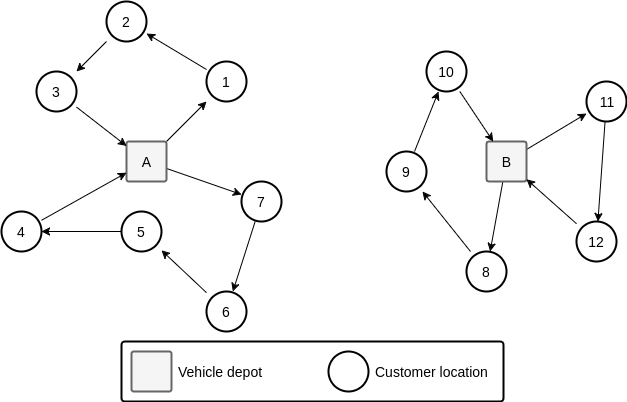
\includegraphics[width=5cm]{Resources/Images/mdvrp-illustration}
	\caption{Ilustrasi \textit{Multi Depot} VRP}
	\label{fig:mdvrp-illustration}
\end{figure}


The MDVRP can be formalized as follows. Let $G = (V, A)$ be a complete graph, where $V$ is the set of nodes and $A$ is the set of arcs. The nodes are partitioned into two subsets: the customers to be served, $V_C$ = \{1,..., $N$\}, and the multiple depots $V_D$ = \{$N$+1,..., $N+M$\}, with $V_C \cup V_D$ = $V$ and $V_C \cap V_D$ = $\oslash$. There is a non-negative cost $c_ij$ associated with each arc $(i, j) \in A$. The demand of each customer is $d_i$ (there is no demand at the depot nodes). There is also a fleet of $K$ identical vehicles, each with capacity $Q$. The service time at each customer $i$ is $t_i$ while the maximum route duration time is set to $T$. $A$ conversion factor $w_{ij}$ might be needed to transform the cost $c_{ij}$ into time units. In this work, however, the cost is the same as the time and distance units, so $w_{ij}$ = $1$.


In the mathematical formulation that follows, binary variables $x_{ijk}$ are equal to $1$ when vehicle $k$ visits node $j$ immediately after node $i$. Auxiliary variables $y_i$ are also used in the subtour elimination constraints.


\begin{equation}
\label{eq:1}
\begin{aligned}
\sum_{i=1}^{N+M}\sum_{j=1}^{N+M}\sum_{k=1}^{K}c_{ij}x_{ijk};
\end{aligned}
\end{equation}

\begin{equation}
\label{eq:2}
\begin{aligned}
\sum_{i=1}^{N+M}\sum_{k=1}^{K}x_{ijk} = 1  (j=1,..., N);
\end{aligned}
\end{equation}

\begin{equation}
\label{eq:3}
\begin{aligned}
\sum_{j=1}^{N+M}\sum_{k=1}^{K}x_{ijk} = 1  (j=1,..., N);
\end{aligned}
\end{equation}

\begin{equation}
\label{eq:4}
\begin{aligned}
\sum_{i=1}^{N+M}x_{ihk} - \sum_{j=1}^{N+M}x_{hjk} = 0 \\
(k=1,...,K; h=1,...,N+M);
\end{aligned}
\end{equation}

\begin{equation}
\label{eq:5}
\begin{aligned}
\sum_{i=1}^{N+M} \sum_{j=1}^{N+M} d_ix_{ijk} \leq Q (k=1,...,K);
\end{aligned}
\end{equation}

\begin{equation}
\label{eq:6}
\begin{aligned}
\sum_{i=1}^{N+M} \sum_{j=1}^{N+M} (c_{ij}w_{ij} + t_i) x_{ijk} \leq T (k=1,...,K);
\end{aligned}
\end{equation}

\begin{equation}
\label{eq:7}
\begin{aligned}
\sum_{i=N+1}^{N+M} \sum_{j=1}^{N} x_{ijk} \leq 1 (k=1,...,K);
\end{aligned}
\end{equation}

\begin{equation}
\label{eq:8}
\begin{aligned}
\sum_{j=N+1}^{N+M} \sum_{i=1}^{N} x_{ijk} \leq 1 (k=1,...,K);
\end{aligned}
\end{equation}

\begin{equation}
\label{eq:9}
\begin{aligned}
y_i - y_j + (M + N)x_{ijk} \leq N + M - 1; \\
for 1 \leq i \neq j \leq N and 1 \leq k \leq K;
\end{aligned}
\end{equation}

\begin{equation}
\label{eq:10}
\begin{aligned}
x_{ijk} \in \{0, 1\} \forall i,j,k;
\end{aligned}
\end{equation}

\begin{equation}
\label{eq:11}
\begin{aligned}
y_i \in \{0,1\} \forall i;
\end{aligned}
\end{equation}


The objective \ref{eq:1} minimizes the total cost. Constraints \ref{eq:2} and \ref{eq:3} guarantee that each customer is served by exactly one vehicle. Flow conservation is guaranteed through constraint \ref{eq:4}. Vehicle capacity and route duration constraints are found in \ref{eq:5} and \ref{eq:6}, respectively. Constraints \ref{eq:7} and \ref{eq:8} check vehicle availability. Subtour elimination constraints are in \ref{eq:9}. Finally, \ref{eq:10} and \ref{eq:11} define x and y as binary variables.


%-----------------------------------------------------------------------------%
\subsection{Evolution Algorithms}
\label{ssec:evolution-algorithms}
%-----------------------------------------------------------------------------%
\textit{Evolution Algorithms (EAs)} merupakan salah satu \textit{family} dari algoritma optimasi yang terinspirasi dari alam. Pada algoritma evolusi, terdapat proses seleksi dan reproduksi untuk memurnikasi populasi dari kandidat solusi \cite{eugster_many_2003}. Secara umum \textit{lifecycle} dari \textit{Evolution Algorithms} diawali dengan  konfigurasi populasi awal secara random. Kemudian, setiap iterasi dimulai dengan evaluasi atas fungsi obyektif atas individu pada populasi. Berdasarkan hasil evaluasi, kemudian \textit{fitness value} disematkan pada setiap kandidat solusi pada populasi. Kandidat solusi tersebut kemudian mengalami reproduksi dan menghasilkan generasi berikutnya. Proses kemudian berulang dengan menggunakan individu generasi yang baru.


Coevolutionary (CoE) algorithms (CoEA), merupakan pengembangan dari EAs. In standard EAs, evolution is usually viewed as if the population attempts to adapt in a fixed physical environment. In contrast, coevolutionary (CoE) algorithms (CoEA) realize that in natural evolution the physical environment is influenced by other independently-acting biological populations \cite{engelbrecht_coevolution_2007}. CoEA dapat dibagi menjadi dua, tergantung interaksi dari masing-masing spesies: \textit{competitive} dan \textit{cooperative}. Pada \textit{competitive coevolution} setiap individu berkompetisi dengan satu kelompoknya. Sementara pada \textit{cooperative coevolution}, interaksi antar spesies bersifat saling menguntungkan, atau paling tidak, tidak saling membahayakan \cite{engelbrecht_coevolution_2007}.


%-----------------------------------------------------------------------------%
\subsection{Publish/Subscribe Paradigm}
\label{ssec:pub-sub}
%-----------------------------------------------------------------------------%
\textit{Publish/subscribe interaction} merupakan salah satu metode komunikasi antara \textit{client} dan \textit{server}. Paradigma interaksi pada \textit{publish/subscribe} adalah adanya \textit{subscriber} yang memiliki ketertarikan pada suatu \textit{event} atau \textit{pattern of event}, agar dapat dikirimkan notifikasi tentang sebuah \textit{event} oleh \textit{publisher} yang sesuai dengan \textit{interest}-nya \cite{eugster_many_2003}.


Model dasar dari sistem \textit{publish/subscribe}, seperti Gambar \ref{fig:pub-sub-general}, bergantung pada \textit{event notification service} yang menyediakan penyimpanan dan \textit{management of subscription}. \textit{Event service} tersebut berperan sebagai mediator antara \textit{publisher} yang berperan sebagai \textit{producer} dari \textit{event} dan \textit{subscriber} yang berperan sebagai \textit{consumer} dari \textit{event}.


\begin{figure}[h]
	\centering
	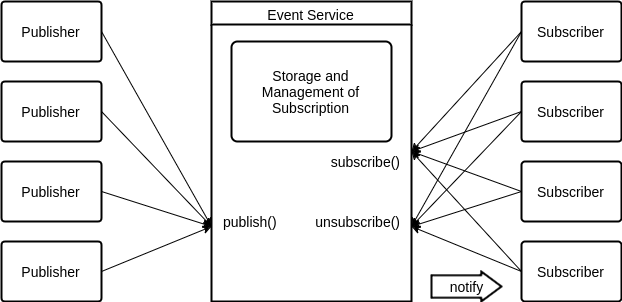
\includegraphics[width=8cm]{Resources/Images/pub-sub-general}
	\caption{Arsitektur dasar pada Pub/Sub \cite{eugster_many_2003}}
	\label{fig:pub-sub-general}
\end{figure}


Salah satu keuntungan dari mekanisme publish/subscribe adalah bersifat loose coupling \cite{eugster_many_2003} antara publisher dengan subscriber. Pemisahan informasi (\textit{decoupling}) yang terjadi antara \textit{subscriber} dan \textit{publisher} dapat dipisahkan dalam 3 (tiga) dimensi, yaitu:

\begin{enumerate}
\item \textit{Space decoupling.} \\
Interaksi antara \textit{publisher} dan \textit{subscriber} tidak perlu saling mengetahui satu dengan yang lain. \textit{Publisher} mengirimkan \textit{event}, dan \textit{subscriber} menerima \textit{event} secara tidak langsung melalui \textit{event service}. \textit{Publisher} biasanya tidak memegang referensi terhadap \textit{subscriber}. Begitu juga sebaliknya, \textit{subscriber} biasanya tidak memegang referensi terhadap \textit{publisher}.
\item \textit{Time decoupling.} \\
Pihak-pihak yang berinteraksi, tidak harus berinteraksi pada waktu yang bersamaan. \textit{Publisher} dapat mengirimkan \textit{event} pada saat \textit{subscriber} dalam kondisi terputus. Begitu juga sebaliknya, \textit{subscriber} tetap dapat menerima \textit{event}, meskipun \textit{original publisher} dalam kondisi terputus.
\item \textit{Synchronizing decoupling.} \\
\textit{Publisher} tidak diblok ketika memproduksi \textit{event}, dan juga \textit{subscriber} tetap dapat memperoleh informasi meskipun sedang mengerjakan tugas yang lain. \textit{Publisher} dan \textit{subscriber} tidak berada dalam \textit{main flow}, sehingga tidak berinteraksi secara \textit{synchronous}.
\end{enumerate}


%-----------------------------------------------------------------------------%
\section{Proposed Solution}
\label{sec:proposed-solution}
%-----------------------------------------------------------------------------%
Kelemahan MDVRP ketika digunakan dalam rekomendasi lokasi pencacahan adalah ketiadaan data service time, padahal data itu sangat penting dalam kalkulasi rekomendasi. Untuk itu, MDVRP perlu diintegrasikan dengan mekanisme real-time. Terdapat beberapa mekanisme yang dapat diadopsi pada real-time system, diantaranya: Web service, RPC, message passing, dan publish/subscribe \cite{eugster_many_2003}. 


Mekanisme publish/subscribe digunakan dalam penelitian ini karena memiliki sifat \textit{loose coupling}. Selain itu mekanisme publish/subscribe juga sesuai sesuai digunakan pada sistem yang bersifat information driven \cite{muhl_large-scale_2002}. Karena karakteristiknya ini, maka publish/subscribe dapat bekerja secara asynchronous, dimana \textit{request} dan \textit{reply} tidak harus diproses secara berurutan. Pada saat \textit{subscriber} melakukan subscribe, publisher tidak harus dalam kondisi online, begitu juga sebaliknya, pada saat \textit{publisher} melakukan publish, \textit{subscriber} tidak harus dalam kondisi online.


\begin{figure}[h]
	\centering
	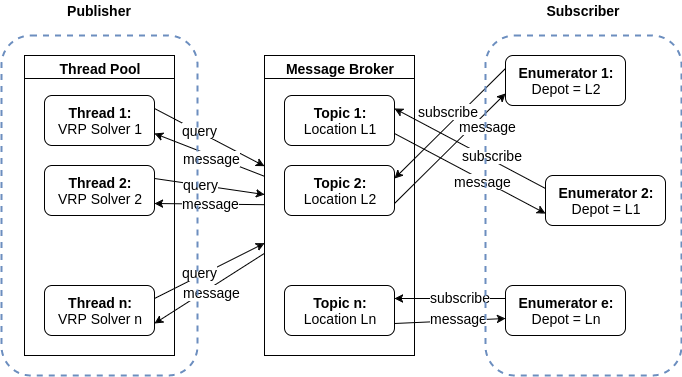
\includegraphics[width=8cm]{Resources/Images/system-overview}
	\caption{Garis Besar Sistem}
	\label{fig:system-overview}
\end{figure}


Gambar \ref{fig:system-overview} menunjukkan garis besar sistem, dimana sistem tersusun atas 3 (tiga) komponen utama, yaitu: \textit{publisher}, \textit{subscriber}, dan \textit{message broker}. Komunikasi antara \textit{publisher} dan \textit{subscriber} didasari atas satu kesamaan, yaitu \textbf{event} atau \textbf{topic}. Topik yang digunakan sebagai dasar komunikasi antara publisher dan subscriber dalam penelitian ini adalah \textit{current location} dari masing-masing subscriber.


%-----------------------------------------------------------------------------%
\subsection{Recommendation Publisher}
\label{ssec:recommendation-publisher}
%-----------------------------------------------------------------------------%
VRP Solver diimplementasikan pada sisi publisher, yang akan melakukan pencarian solusi/rute dan kemudian dipublish kepada \textit{subscriber} melalui \textit{message broker}. Sebagaimana sebelumnya disebutkan, bahwasannya \textit{current location} dari masing-masing \textit{subscriber} digunakan sebagai topik. Sebuah thread disiapkan, yang secara periodik akan melakukan pengecekan apakah terdapat topik yang baru pada message broker.


Setiap kali terdapat topik yang baru, sebuah thread akan disiapkan, dan topik tersebut digunakan sebagai ID dari thread yang bersangkutan. Pada thread tersebut terdapat procedure VRP solver yang akan melakukan pencarian solusi/rute. Untuk itu, sebuah threadpool disiapkan untuk menampung thread dari masing-masing topik tersebut secara berurutan berdasarkan kedatangan. Karena topik digunakan sebagai thread ID, maka ukuran dari threadpool akan sama dengan jumlah seluruh lokasi pencacahan.


Setiap thread dalam threadpool kemudian dijalankan secara berurutan, satu session untuk masing-masing thread. Setiap thread yang dijalankan, yang menggunakan topik sebagai ID, akan melakukan pencarian solusi dengan melibatkan seluruh $M$ vehicles dan $(unassigned) N$ locations. Pencarian solusi dilakukan pada procedure VRP solver pada section \ref{ssec:vrp-solver}.


\begin{algorithm}[h]
	\caption{TopicWatcher}
	\begin{algorithmic}[1]
		\renewcommand{\algorithmicrequire}{\textbf{Input:}}
		\renewcommand{\algorithmicensure}{\textbf{Output:}}
		\REQUIRE $C$
		\ENSURE  $T$
		\FOR {$i = 1$ to $len(C)$}
			\FOR {$j = 1$ to $N$}
				\IF {($C_i == E_j$)}
					\STATE $T_j = Thread(C_i, V_1...V_M, (unassigned) E_1...E_N)$
				\ENDIF
			\ENDFOR
		\ENDFOR
		\RETURN $T$
	\end{algorithmic}
\end{algorithm}


Proses dalam procedure VRP solver pada masing-masing thread akan menghasilkan sejumlah minimal $1$ rute, dan maksimal $M$ rute. Setiap rute $R_i$ yang dihasilkan kemudian akan dipublish dengan topik $C_i$. Setelah rute dipublish, \textit{message broker} akan menginformasikan kepada publisher, jumlah \textit{subscriber} yang menerima pesan. Adapun identitas \textit{subscriber} yang menerima pesan tetap tidak diketahui oleh \textit{publisher}.


Setiap rute $R_i$ yang memiliki jumlah penerima pesan lebih dari satu, maka \textit{thread} yang mempunyai ID $C_{R_i}$ akan dicancel. Pembatalan \textit{thread} ini dimaksudkan agar solusi/rute yang telah diterima oleh \textit{subscriber} tidak dikalkulasi kembali. Terdapat sebuah kondisi, dimana pada saat thread menjalankan VRPSolver dengan ID $C_i$, ternyata rute yang dihasilkan tidak mengandung solusi untuk topik $C_i$. Pada kondisi tersebut, maka topik $C_i$ tersebut akan diantrikan kembali dengan hanya menyertakan dirinya sendiri sebagai pencacah, sehingga diperoleh kepastian topik $C_i$ akan memperoleh solusi/rute.


\begin{algorithm}[h]
	\caption{VRPWorker}
	\label{alg:vrp-worker}
	\begin{algorithmic}[1]
		\renewcommand{\algorithmicrequire}{\textbf{Input:}}
		\renewcommand{\algorithmicensure}{\textbf{Output:}}
		\REQUIRE $T$
		\ENSURE  $R$
		\FOR {$i = 1$ to $len(T)$}
			\STATE $R$ = VRPSolver($T_i$)
			\FOR {$j = 1$ to $len(R)$}
				\STATE $r$ = publish($C_{R_j}$, $R_j$)
				\IF {($r > 0$)}
					\STATE cancelSolver($T_j$)
				\ELSIF {($C_{T_i} \notin C_{R_j}$)}
					\STATE $T_i = Thread(C_{T_i}, V_m, (unassigned) E_1...E_N)$
				\ENDIF
			\ENDFOR
		\ENDFOR
		\RETURN $R$
	\end{algorithmic}
\end{algorithm}


Salah satu keuntungan mekanisme publish/subscribe, yang membuat dia fleksible, adalah karakteristiknya yang loose coupling. Dalam kasus ini, keuntungan dari mekanisme ini sekaligus menjadi kelemahan. Ketidaktahuan \textit{publisher} akan identitas \textit{subscriber} menyebabkan \textit{current location} dari keseluruhan \textit{subscriber} tidak dapat diketahui. Untuk itu diperlukan mekanisme yang dapat mengatasi permasalahan pertukaran identitas, yaitu dengan menggunakan \textit{shared memory}. Pada \textit{shared memory} tersimpan data \textit{current location} dari seluruh \textit{subscriber}, yang mana \textit{publisher} dapat mengetahui \textit{current location} dari seluruh \textit{subscriber} dari data yang tersimpan pada \textit{shared memory}.


Proses tersebut diatas terus berulang, sampai dengan seluruh lokasi pencacahan semuanya ter-assign. Gambar \ref{fig:publisher-algorithm} memberikan ilustrasi algoritma yang digunakan pada \textit{recommendation publisher}.


\begin{figure}[h]
	\centering
	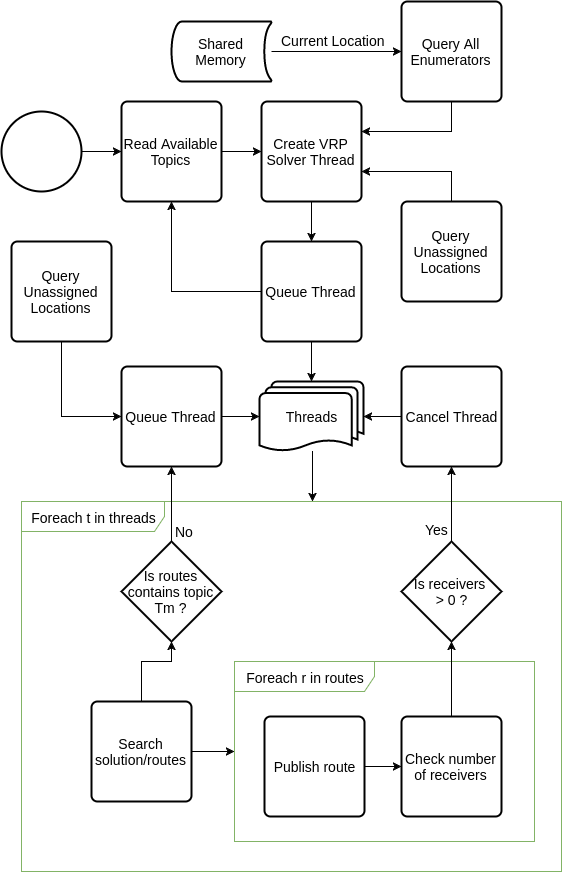
\includegraphics[width=8cm]{Resources/Images/publisher-algorithm}
	\caption{Publisher Workflow}
	\label{fig:publisher-algorithm}
\end{figure} 


%-----------------------------------------------------------------------------%
\subsection{VRP Solver}
\label{ssec:vrp-solver}
%-----------------------------------------------------------------------------%
VRP Solver merupakan module yang digunakan untuk melakukan pencarian solusi/rute yang akan dikunjungi. VRP Solver dipanggil pada setiap thread yang terdapat pada threadpool \ref{alg:vrp-worker}. Terdapat beberapa algoritma yang dapat digunakan dalam pencarian solusi pada MDVRP, antara lain: tabu search \cite{cordeau_tabu_1997}, adaptive large neighborhood search  \cite{pisinger_general_2007}, fuzzy logic guided genetic algorithm \cite{lau_application_2010}, paralel iterated tabu search \cite{cordeau_parallel_2012}, hybrid algorithm combining Iterated Local Search and Set Partitioning \cite{subramanian_hybrid_2013}, hybrid genetic algorithm with adaptive diversity control \cite{vidal_implicit_2014}, hybrid Granular Tabu Search \cite{escobar_hybrid_2014}, dan \textit{Evolution Algorithms (EAs)} \cite{de_oliveira_cooperative_2016}. Pada kasus ini akan digunakan coevolutionary algoritma CoEAs, karena CoEAs menghasilkan \textit{mean solution values} yang competitive dengan \textit{CPU time} yang relatif lebih rendah dibandingkan algoritma yang lain \cite{de_oliveira_cooperative_2016}.


Langkah-langkah yang dilakukan pada VRP Solver yang mengadopsi algoritma CoEAs adalah sebagai berikut
\begin{enumerate}
\item Create problem \\
MDVRP problem yang akan disusun terdiri dari sejumlah vehicle $V$ dan sejumlah edge $E$ yang telah diassign pada masing-masing thread.
\item Decompose problem. \\
MDVRP problem didecompose memjadi beberapa subproblem.
\item Evolve. \\
Masing-masing individu pada setiap subproblem kemudian berevolusi. Setiap evolusi berakhir, individu baru akan dievaluasi. Jika individu baru yang terbentuk lebih baik, maka solusi diterima, dan individu-individu terbaik diupdate. Evolusi akan terus berlangsung sampai stop kriteria terpenuhi. Stop kriteria yang digunakan adalah waktu. Evolusi akan berhenti ketika total waktu mencapai 60 detik, atau 40 detik tanpa perubahan individu terbaik.
\end{enumerate}


\begin{algorithm}[h]
	\caption{VRPWorker}
	\begin{algorithmic}[1]
		\renewcommand{\algorithmicrequire}{\textbf{Input:}}
		\renewcommand{\algorithmicensure}{\textbf{Output:}}
		\REQUIRE $T_i$
		\ENSURE  $R$
		\STATE P $\leftarrow$ createProblem($V_1...V_{T_i}$, $E_1...E_{T_i}$)
		\\ \textit{Decompose problem into S subproblem}
		\STATE SP $\leftarrow$ decomposeProblem(P)
		\WHILE {stopCriteriaUnmet}
			\FOR {$i=1$ to $len(SP)$}
				\STATE I $\leftarrow$ $SP_i \rightarrow individuals$
				\FOR {$j$ to $len(I)$}
					%\\ \textit{Foreach individu in subpopulation, do evolve}
					\STATE $O_j$ $\leftarrow$ $I_j \rightarrow evolve()$
				\ENDFOR
				\STATE shrink($I$, $O$)
			\ENDFOR
			%\\ \textit{Every iteration, update best individuals}
			\STATE updateBestIndividuals()
		\ENDWHILE
		\STATE $B \leftarrow getBestIndividuals()$ 
		\STATE $R \leftarrow convert(B)$ 
		\RETURN $R$
	\end{algorithmic}
\end{algorithm}


%-----------------------------------------------------------------------------%
\subsection{Message Broker}
\label{ssec:message-broker}
%-----------------------------------------------------------------------------%
\textit{Message broker} adalah sebuah komponen yang bertanggung jawab dalam menyalurkan (\textit{routing}) pesan dari \textit{publisher} ke \textit{subscriber} sesuai dengan topik yang di\textit{subscribe} \cite{banavar_efficient_1999}. Suatu sistem \textit{publish/subscribe} dapat memiliki \textit{single broker} maupun \textit{multi broker}. Pada arsitektur \textit{single broker}, seluruh \textit{subscriber} dan \textit{publisher} terkoneksi pada satu \textit{broker}, sementara pada \textit{multi broker}, setiap \textit{subscriber} maupun \textit{publisher} dapat terkoneksi pada broker terdekat. Arsitektur \textit{multi depot} ini juga disebut dengan \textit{distributed pub/sub system} \cite{muhl_large-scale_2002}, seperti ilustrasi pada Gambar \ref{fig:pub_sub_distributed_ilustration}. Adapun rancangan yang diusulkan akan menerapkan arsitektur terdistribusi, dikarenakan lokasi pencacahan secara geografis tersebar.


\begin{figure}[h]
	\centering
	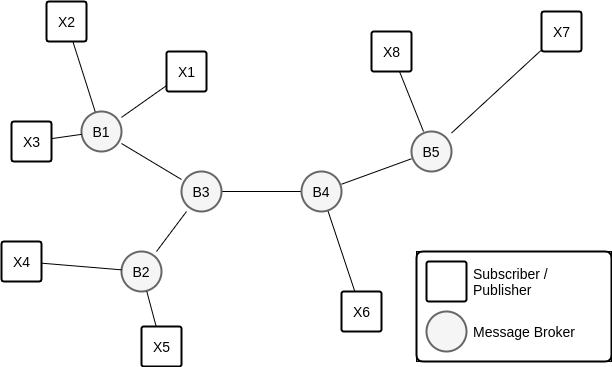
\includegraphics[width=7cm]{Resources/Images/pub_sub_distributed_ilustration}
	\caption{Arsitektur \textit{Publish-Subscribe} terdistribusi}
	\label{fig:pub_sub_distributed_ilustration}
\end{figure}


%-----------------------------------------------------------------------------%
\section{Testing}
\label{sec:testing}
%-----------------------------------------------------------------------------%
The performance of the proposed system was assessed through a number of experiments. Eksperimen ini menggunakan dua macam data: Cordeau and data field. Service time pada kedua macam data tersebut akan digenerate secara random dengan mengikuti distribusi normal.


\begin{enumerate}
\item Data yang diambil dari Cordeau \cite{cordeau_tabu_1997}, terdiri dari 50 \textit{customers} dan 4 \textit{vehicles}. Jarak antar lokasi dihitung dengan cara euclidean.
\item Data yang diambil dari kondisi real lapangan, yang terdiri dari 182 \textit{customers} dan 15 \textit{vehicles}. Jarak dan durasi antar lokasi diukur dengan bantuan Google Direction API.
\end{enumerate}


Data yang akan digunakan, Cordeau type 2 dan data lapangan, akan diujicobakan dengan menggunakan program usulan, berbasis Pub/Sub dan CoES. Data kemudian diperbandingkan dengan program pembanding yang mengimplementasi algoritma CoES tanpa mekanisme Pub/Sub. Dari kedua program tersebut akan diperoleh output rute untuk masing-masing \textit{vehicle} dengan ilustrasi sebagi berikut:

\begin{itemize}
\item \textit{Vehicle} A = Loc1 $\rightarrow$ Loc5 $\rightarrow$ Loc15 $\rightarrow$ Loc6
\item \textit{Vehicle} B = Loc 6 $\rightarrow$ Loc2 $\rightarrow$ Loc16 $\rightarrow$ Loc3
\item \textit{Vehicle} C = Loc4 $\rightarrow$ Loc8 $\rightarrow$ Loc14 $\rightarrow$ Loc 7
\item \textit{Vehicle} D = Loc9 $\rightarrow$ Loc10 $\rightarrow$ Loc11 $\rightarrow$ Loc12
\end{itemize}


Masing-masing rute kemudian dihitung \textit{total cost}-nya, yang merupakan penjumlahan dari seluruh \textit{service time} pada masing-masing lokasi dan seluruh waktu tempuh dari masing-masing perpindahan. Metric yang akan dijadikan pembanding adalah standar deviasi dari seluruh rute pada masing-masing program dan program pembanding. Program yang lebih baik akan menghasilkan standar deviasi yang lebih kecil. Standar deviasi dipilih sebagai \textit{metric} karena merepresentasikan kondisi sebenarnya dilapangan, dimana jika variasi waktu dari seluruh pencacah lebih kecil, maka penyelesaian pencacahan akan lebih merata.


Pada pengujian kondisi normal dengan menggunakan data Cordeau, diperoleh hasil bahwasannya pre-calculated routes dengan menggunakan algoritma CoES menghasilkan total time yang lebih kecil, yaitu 1165513.28 seconds berbanding 1165706.84 seconds untuk Pub/Sub + CoES, namun menghasilkan standar deviasi yang jauh lebih besar, yaitu 98268.51 seconds berbading 12997.91 seconds (Table \ref{tbl:test_result_normal_cordeau_comparison}). Sementara pengujian kondisi normal dengan menggunakan data lapangan, diperoleh hasil bahwasannya pre-calculated routes dengan menggunakan algoritma CoES menghasilkan total time yang lebih kecil, yaitu 4448989.67 seconds berbanding 4559658.67 seconds untuk Pub/Sub + CoES, namun menghasilkan standar deviasi yang jauh lebih besar, yaitu 119720.84 seconds berbading 34472.12 seconds (Table \ref{tbl:test_result_normal_field_comparison}).


\begin{table}
	\centering
	\ra{1.3}
	\caption{Komparasi CoES dan Pub/Sub + CoES pada Data Cordeau}
	\label{tbl:test_result_normal_cordeau_comparison}
	\begin{tabular}{lrr}
		\toprule
			Ukuran & CoES & CoES + Pub/Sub\\ 
		\midrule
			Total time & 1165513.28 & 1165706.84\\
			Mean of time & 291378.32 & 291426.71\\
			Std. Dev of time & 98268.51 & 12997.91\\
		\bottomrule
	\end{tabular}
\end{table}


\begin{table}
	\centering
	\ra{1.3}
	\caption{Komparasi CoES dan Pub/Sub + CoES pada Data Lapangan}
	\label{tbl:test_result_normal_field_comparison}
	\begin{tabular}{lrr}
		\toprule
			Ukuran & CoES & CoES + Pub/Sub\\ 
		\midrule
			Total Waktu & 4448989.67 & 4559658.67\\
			Rata-rata & 296599.31 & 303977.24\\
			Standar Deviasi & 119720.84 & 34472.12\\
		\bottomrule
	\end{tabular}
\end{table}


%-----------------------------------------------------------------------------%
\section{Conclusion and Future Works}
\label{sec:conclusion-future-works}
%-----------------------------------------------------------------------------%
Paper ini mengusulkan penggunaan Cooperative Coevolutionary Algorithm (CoES) yang dikombinasikan dengan mekanisme Publish/Subscribe untuk mengatasi permasalahan rekomendasi lokasi pengumpulan data secara real-time. Dari hasil pengujian diperoleh hasil bahwasannya pre-calculated routes yang dihasilkan dengan algoritma CoES menghasilkan total route times lebih kecil daripada CoES Pub/Sub. Akan tetapi, algoritma CoES Pub/Sub menghasilkan standar deviasi yang lebih kecil dari pada CoES, yang artinya beban yang dialokasikan untuk setiap petugas lebih merata.




% An example of a floating figure using the graphicx package.
% Note that \label must occur AFTER (or within) \caption.
% For figures, \caption should occur after the \includegraphics.
% Note that IEEEtran v1.7 and later has special internal code that
% is designed to preserve the operation of \label within \caption
% even when the captionsoff option is in effect. However, because
% of issues like this, it may be the safest practice to put all your
% \label just after \caption rather than within \caption{}.
%
% Reminder: the "draftcls" or "draftclsnofoot", not "draft", class
% option should be used if it is desired that the figures are to be
% displayed while in draft mode.
%
%\begin{figure}[!t]
%\centering
%\includegraphics[width=2.5in]{myfigure}
% where an .eps filename suffix will be assumed under latex, 
% and a .pdf suffix will be assumed for pdflatex; or what has been declared
% via \DeclareGraphicsExtensions.
%\caption{Simulation results for the network.}
%\label{fig_sim}
%\end{figure}

% Note that the IEEE typically puts floats only at the top, even when this
% results in a large percentage of a column being occupied by floats.


% An example of a double column floating figure using two subfigures.
% (The subfig.sty package must be loaded for this to work.)
% The subfigure \label commands are set within each subfloat command,
% and the \label for the overall figure must come after \caption.
% \hfil is used as a separator to get equal spacing.
% Watch out that the combined width of all the subfigures on a 
% line do not exceed the text width or a line break will occur.
%
%\begin{figure*}[!t]
%\centering
%\subfloat[Case I]{\includegraphics[width=2.5in]{box}%
%\label{fig_first_case}}
%\hfil
%\subfloat[Case II]{\includegraphics[width=2.5in]{box}%
%\label{fig_second_case}}
%\caption{Simulation results for the network.}
%\label{fig_sim}
%\end{figure*}
%
% Note that often IEEE papers with subfigures do not employ subfigure
% captions (using the optional argument to \subfloat[]), but instead will
% reference/describe all of them (a), (b), etc., within the main caption.
% Be aware that for subfig.sty to generate the (a), (b), etc., subfigure
% labels, the optional argument to \subfloat must be present. If a
% subcaption is not desired, just leave its contents blank,
% e.g., \subfloat[].


% An example of a floating table. Note that, for IEEE style tables, the
% \caption command should come BEFORE the table and, given that table
% captions serve much like titles, are usually capitalized except for words
% such as a, an, and, as, at, but, by, for, in, nor, of, on, or, the, to
% and up, which are usually not capitalized unless they are the first or
% last word of the caption. Table text will default to \footnotesize as
% the IEEE normally uses this smaller font for tables.
% The \label must come after \caption as always.
%
%\begin{table}[!t]
%% increase table row spacing, adjust to taste
%\renewcommand{\arraystretch}{1.3}
% if using array.sty, it might be a good idea to tweak the value of
% \extrarowheight as needed to properly center the text within the cells
%\caption{An Example of a Table}
%\label{table_example}
%\centering
%% Some packages, such as MDW tools, offer better commands for making tables
%% than the plain LaTeX2e tabular which is used here.
%\begin{tabular}{|c||c|}
%\hline
%One & Two\\
%\hline
%Three & Four\\
%\hline
%\end{tabular}
%\end{table}


% Note that the IEEE does not put floats in the very first column
% - or typically anywhere on the first page for that matter. Also,
% in-text middle ("here") positioning is typically not used, but it
% is allowed and encouraged for Computer Society conferences (but
% not Computer Society journals). Most IEEE journals/conferences use
% top floats exclusively. 
% Note that, LaTeX2e, unlike IEEE journals/conferences, places
% footnotes above bottom floats. This can be corrected via the
% \fnbelowfloat command of the stfloats package.


% conference papers do not normally have an appendix


% use section* for acknowledgment
% \section*{Acknowledgment}
% The authors would like to thank...





% trigger a \newpage just before the given reference
% number - used to balance the columns on the last page
% adjust value as needed - may need to be readjusted if
% the document is modified later
%\IEEEtriggeratref{8}
% The "triggered" command can be changed if desired:
%\IEEEtriggercmd{\enlargethispage{-5in}}

% references section

% can use a bibliography generated by BibTeX as a .bbl file
% BibTeX documentation can be easily obtained at:
% http://mirror.ctan.org/biblio/bibtex/contrib/doc/
% The IEEEtran BibTeX style support page is at:
% http://www.michaelshell.org/tex/ieeetran/bibtex/
% bibliographystyle{IEEEtran}
% argument is your BibTeX string definitions and bibliography database(s)
% bibliography{IEEEabrv,Paper.bib}
%
% <OR> manually copy in the resultant .bbl file
% set second argument of \begin to the number of references
% (used to reserve space for the reference number labels box)
% \begin{thebibliography}{1}

% \bibitem{IEEEhowto:kopka}
% H.~Kopka and P.~W. Daly, \emph{A Guide to \LaTeX}, 3rd~ed.\hskip 1em plus
%   0.5em minus 0.4em\relax Harlow, England: Addison-Wesley, 1999.

% \end{thebibliography}

\bibliographystyle{IEEEtran}
\bibliography{Resources/Bib/Reference}


% that's all folks
\end{document}


